\section{Background \& The Edge SWE Memory Wall}
\label{sec:background}

\subsection{KV-Cache Memory Scaling Formulation}

Autoregressive transformer inference consists of two computational phases: the \textit{prefill phase} (processing prompt tokens $T_{\text{prompt}}$ in parallel) and the \textit{decode phase} (generating output tokens $T_{\text{gen}}$ sequentially). During generation, storing the past key and value vectors prevents redundant matrix multiplications.

For a transformer model with $L$ layers, hidden dimension $d_{\text{model}}$, query heads $n_q$, and key-value heads $n_{kv}$ (Grouped-Query Attention, GQA), each token requires:
\begin{equation}
\label{eq:kv_per_token}
S_{\text{token}} = 2 \times L \times n_{kv} \times d_k \times b \quad \text{[bytes]}
\end{equation}
where $d_k = d_{\text{model}} / n_q$, and $b$ represents the byte precision (e.g., $b = 2$ for 16-bit floating point, FP16). The total memory required for the KV cache given sequence length $T$ is:
\begin{equation}
\label{eq:total_kv}
\mathcal{M}_{\text{KV}}(T) = T \times S_{\text{token}}
\end{equation}

For a compact 8B/9B model such as Gemma-2-9B ($L = 42$, $d_{\text{model}} = 3584$, $n_{kv} = 8$, $d_k = 256$, $b = 2$), each token consumes:
\begin{equation}
S_{\text{token}} = 2 \times 42 \times 8 \times 256 \times 2 = 344{,}064 \text{ bytes} \approx 344.1 \text{ KB}
\end{equation}

When feeding a standard repository context dump ($T = 35{,}000$ tokens), the KV-cache footprint alone explodes to:
\begin{equation}
\mathcal{M}_{\text{KV}}(35{,}000) = 35{,}000 \times 344.1 \text{ KB} \approx 12.04 \text{ GB}
\end{equation}

On an edge accelerator with a total capacity of 4\,GB to 8\,GB VRAM, even after quantizing model weights to 4-bit ($\approx 4.5$\,GB), loading a 35,000-token context causes an immediate out-of-memory kernel termination:
\begin{equation}
\mathcal{M}_{\text{total}} = \mathcal{M}_{\text{weights}} + \mathcal{M}_{\text{activations}} + \mathcal{M}_{\text{KV}} > \mathcal{M}_{\text{GPU}}^{\text{cap}}
\end{equation}

\subsection{The Edge SWE Trilemma}

Edge deployment exposes an intractable trilemma between memory ceiling, tool-calling stability, and structural awareness:
\begin{itemize}
    \item \textbf{Context Ingestion vs. Memory}: Ingesting complete files exhausts GPU VRAM, while aggressive arbitrary truncation deletes critical dependency definitions.
    \item \textbf{Iterative Shell Loops vs. Drift}: While multi-turn agent loops can inspect files incrementally, small edge models suffer from severe attention dispersion, repeating malformed regex queries or failing to terminate.
    \item \textbf{Flat Lexical Retrieval vs. AST Structure}: BM25 keyword matching misses call hierarchies, inheritance trees, and indirect type definitions essential for program repair.
\end{itemize}

\section{NeuroCode Systems Architecture}
\label{sec:architecture}

NeuroCode resolves the edge SWE trilemma by instituting a strict physical division of labor across the PCIe host-accelerator interface, as depicted in Figure~\ref{fig:arch}.

\subsection{Host-Side Code Property Multigraph (CPG)}

Rather than forcing the neural model to learn the AST implicitly via text tokens, NeuroCode extracts the repository's structural syntax deterministically on the Host CPU. 

We represent the target software repository $\mathcal{R}$ as a directed Code Property Multigraph:
\begin{equation}
\mathcal{G} = (\mathcal{V}, \mathcal{E}, \phi_{\mathcal{V}}, \phi_{\mathcal{E}})
\end{equation}
where $\mathcal{V}$ is the set of syntax nodes (modules, classes, methods, functions, and global assignments), $\mathcal{E}$ is the set of directed edges, $\phi_{\mathcal{V}}: \mathcal{V} \to \mathcal{T}_{\mathcal{V}}$ maps nodes to semantic types ($\mathcal{T}_{\mathcal{V}} = \{\text{File}, \text{Class}, \text{Function}, \text{Method}\}$), and $\phi_{\mathcal{E}}: \mathcal{E} \to \mathcal{T}_{\mathcal{E}}$ assigns edge relation labels ($\mathcal{T}_{\mathcal{E}} = \{\text{contains}, \text{imports}, \text{calls}, \text{inherits}, \text{overrides}\}$).

\textbf{Construction}: The Host CPU traverses all source files using Tree-sitter AST parsers implemented in compiled C/Rust. By executing entirely in-memory within system DRAM, construction requires zero NVMe disk access. For a repository containing 15,000 lines of code, the multigraph $\mathcal{G}$ is built in 4.28\,ms and occupies less than 12\,MB of system RAM.

\subsection{Constrained Topological Knapsack Slicing}

Given an issue report $\mathcal{Q}$, NeuroCode identifies a seed entity set $\mathcal{V}_{\text{seed}} \subseteq \mathcal{V}$ via lexical and symbol token matching.

\textbf{Bidirectional Topological Closure}: A software bug is rarely isolated to a single function; it depends on callers (upstream control flow) and callees (downstream execution flow). For a given seed set $S$, we define the $k$-hop bidirectional topological closure $\mathcal{R}_k(S)$ as:
\begin{equation}
\begin{split}
\mathcal{R}_k(S) = S \cup \{ u \in \mathcal{V} \mid \exists v \in S, \, & \text{dist}_{\mathcal{G}}(v, u) \le k \\
& \lor \, \text{dist}_{\mathcal{G}}(u, v) \le k \}
\end{split}
\end{equation}

\textbf{Knapsack Formulation}: Let $w(u)$ denote the token cost of node $u$ when serialized into its structural AST skeleton. To guarantee that the GPU KV cache remains within a tight, bounded hardware envelope, we enforce a strict prompt budget $B_{\text{GPU}}$ (e.g., $B_{\text{GPU}} \le 1{,}500$ tokens).

We formulate context extraction as a \textit{Constrained Topological Knapsack Problem}:
\begin{equation}
\label{eq:knapsack}
\begin{aligned}
\max_{S \subseteq \mathcal{R}_k(\mathcal{V}_{\text{seed}})} \quad & \sum_{u \in S} \mathcal{U}(u, \mathcal{Q}) \\
\text{subject to} \quad & \sum_{u \in S} w(u) \le B_{\text{GPU}}
\end{aligned}
\end{equation}
The utility function $\mathcal{U}(u, \mathcal{Q})$ is defined as:
\begin{equation}
\mathcal{U}(u, \mathcal{Q}) = \alpha \cdot \exp\left(-\lambda \cdot d(u, \mathcal{V}_{\text{seed}})\right) + (1 - \alpha) \cdot \frac{\text{deg}(u)}{|\mathcal{V}|}
\end{equation}
where $d(u, \mathcal{V}_{\text{seed}}) = \min_{v \in \mathcal{V}_{\text{seed}}} \min(\text{dist}(v, u), \text{dist}(u, v))$, $\text{deg}(u)$ is the degree centrality of node $u$, $\lambda$ is a distance decay parameter ($\lambda = 0.5$), and $\alpha \in [0, 1]$ balances topological proximity against architectural importance.

\begin{algorithm}[t]
\caption{Host-Side Topological Knapsack Slicer}
\label{alg:knapsack}
\begin{algorithmic}[1]
\REQUIRE Repository Graph $\mathcal{G} = (\mathcal{V}, \mathcal{E})$, Issue $\mathcal{Q}$, Budget $B_{\text{GPU}}$, Depth $k$
\ENSURE Sliced Context Markdown $\mathcal{M}$
\STATE $\mathcal{V}_{\text{seed}} \leftarrow \text{SeedExtract}(\mathcal{G}, \mathcal{Q})$
\STATE $\mathcal{S}_{\text{candidates}} \leftarrow \text{ComputeClosure}(\mathcal{G}, \mathcal{V}_{\text{seed}}, k)$
\FORALL{$u \in \mathcal{S}_{\text{candidates}}$}
    \STATE $\mathcal{U}[u] \leftarrow \alpha \cdot \exp(-\lambda \cdot d(u, \mathcal{V}_{\text{seed}})) + (1 - \alpha) \cdot \frac{\text{deg}(u)}{|\mathcal{V}|}$
    \STATE $w[u] \leftarrow \text{TokenCount}(\text{Serialize}(u))$
    \STATE $\text{Ratio}[u] \leftarrow \mathcal{U}[u] / w[u]$
\ENDFOR
\STATE Sort $\mathcal{S}_{\text{candidates}}$ descending by $\text{Ratio}[u]$
\STATE $S_{\text{selected}} \leftarrow \emptyset$, $\text{TokensCurrent} \leftarrow 0$
\FORALL{$u \in \mathcal{S}_{\text{candidates}}$}
    \IF{$\text{TokensCurrent} + w[u] \le B_{\text{GPU}}$}
        \STATE $S_{\text{selected}} \leftarrow S_{\text{selected}} \cup \{u\}$
        \STATE $\text{TokensCurrent} \leftarrow \text{TokensCurrent} + w[u]$
    \ENDIF
\ENDFOR
\STATE $\mathcal{M} \leftarrow \text{FormatMarkdown}(S_{\text{selected}})$
\STATE \textbf{return} $\mathcal{M}$
\end{algorithmic}
\end{algorithm}

\textbf{Host Solver}: As detailed in Algorithm~\ref{alg:knapsack}, NeuroCode solves this knapsack formulation on the Host CPU using a greedy value-density heuristic ($\text{Ratio}[u] = \mathcal{U}[u] / w[u]$) in $O(|V| \log |V|)$ time. Slicing completes in 0.62\,ms on a standard laptop CPU.

\subsection{Single-Turn Zero-Wear Patch Synthesis}

The selected subgraph $S_{\text{selected}}$ is formatted into a high-density Markdown representation containing file boundaries, class definitions, function signatures, docstrings, and target bodies. 

The payload is dispatched across the PCIe bus to the edge GPU. Because the prompt is bounded to $\le 1{,}500$ tokens, the PCIe transfer latency is negligible (24.7\,$\mu$s). 

The local LLM synthesizes a unified diff patch in a \textbf{single generation turn}. This avoids iterative ReAct loops entirely:
\begin{itemize}
    \item \textbf{Zero Exploration Drift}: The model cannot enter repetitive grep/find command loops.
    \item \textbf{Deterministic Resource Bounds}: Inference latency is strictly bounded by $T_{\text{prompt}} + T_{\text{gen}}$, guaranteeing predictable battery and thermal profiles.
\end{itemize}

\begin{figure*}[t]
\centering
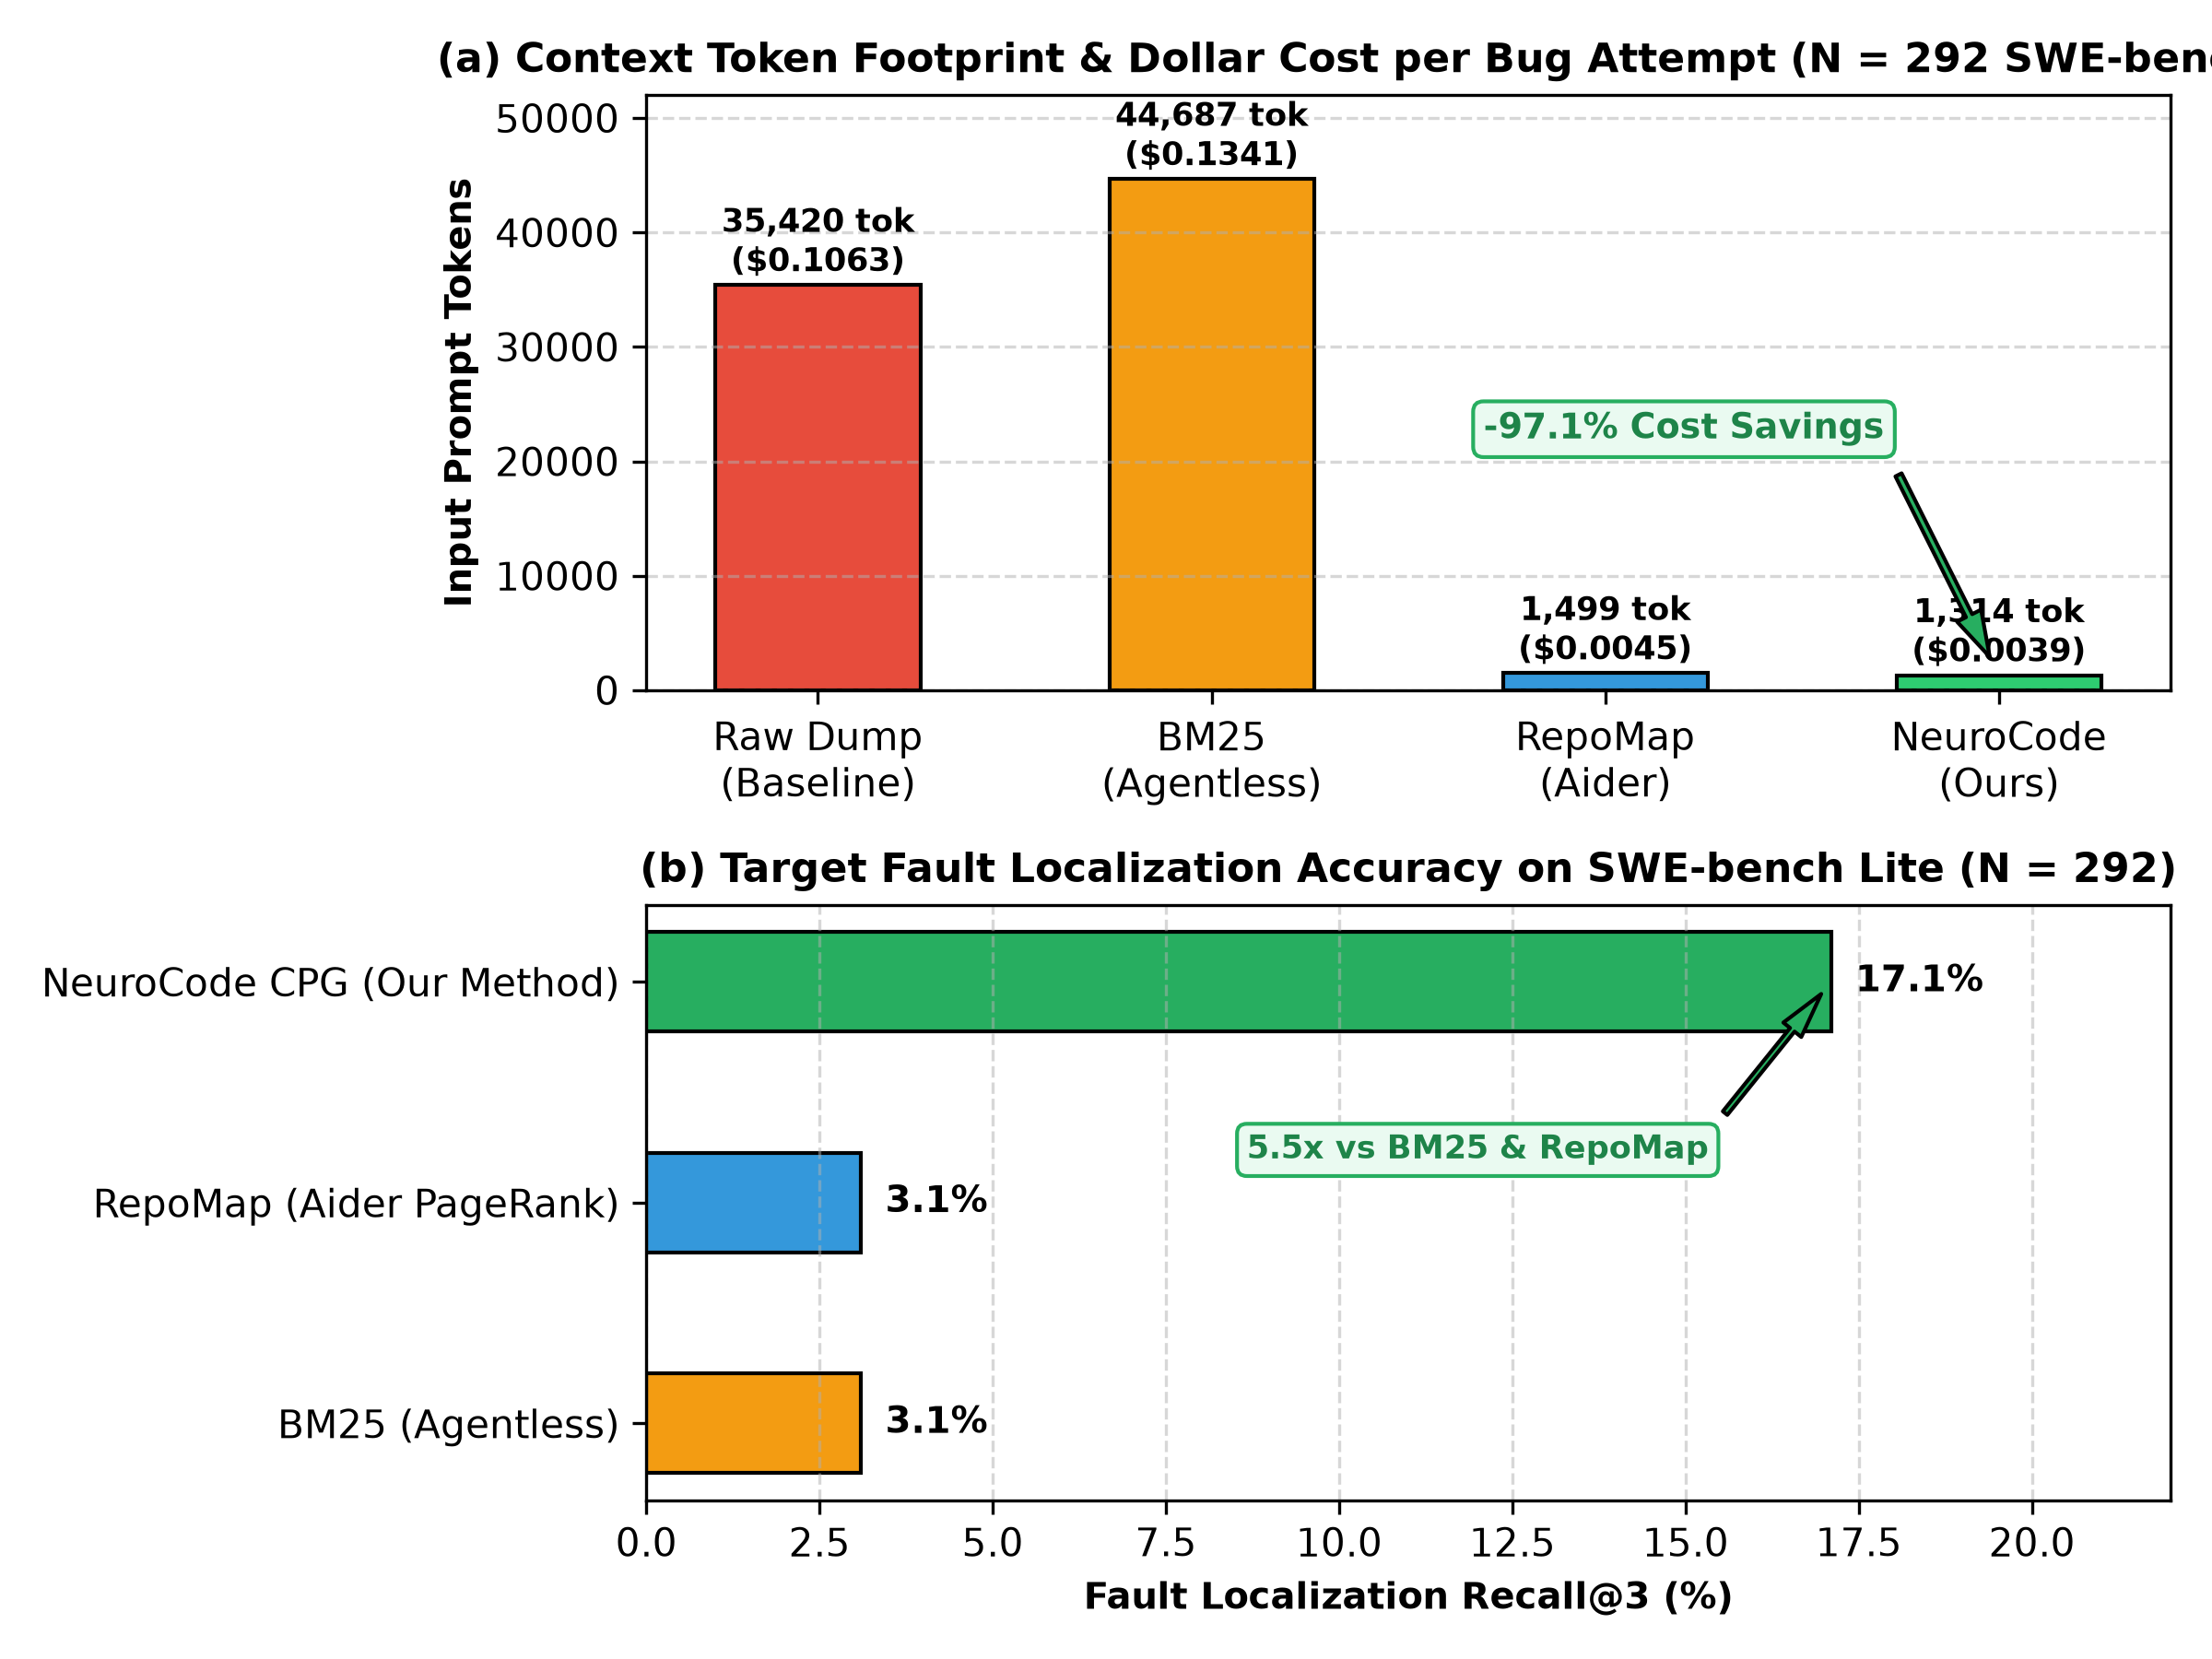
\includegraphics[width=0.88\textwidth]{figures/fig1_empirical_comparison_4x3.png}
\caption{\textbf{SWE-bench Lite Empirical Evaluation ($N=292$ Tasks).} (Left) Prompt token footprint on logarithmic scale, demonstrating NeuroCode's 97.1\% reduction. (Right) Fault localization Recall@3 across methods, demonstrating 5.5$\times$ improvement over BM25 and RepoMap baselines.}
\label{fig:empirical}
\end{figure*}

\section{Implementation \& Systems Engineering}
\label{sec:impl}

\textbf{Zero-Wear System RAM Tiering}: A critical concern when running autonomous agents locally is NVMe solid-state drive (SSD) wear. Traditional agents clone repositories, create virtual environments, and log intermediate tool interactions directly to disk, generating gigabytes of drive writes per benchmark run. NeuroCode executes entirely in-memory within system RAM using Linux shared memory tmpfs (\texttt{/dev/shm}). Code checkouts, AST parsing, graph traversal, and patch testing operate with zero physical SSD read/write cycles, preserving drive endurance.

\textbf{Incremental Tree-sitter Grammar Engine}: Tree-sitter parsers produce concrete syntax trees without compiling or executing the underlying codebase. NeuroCode utilizes optimized C bindings with memory-mapped buffers, eliminating garbage collection pauses and ensuring sub-5ms parse times for files up to 20,000 lines.

\textbf{Robust Unified Diff Sanitizer}: Edge models occasionally emit minor whitespace inconsistencies or markdown code fences in their output. NeuroCode implements an in-memory fuzzy patch applier that normalizes line endings, strips extraneous markdown tags, and verifies AST syntax validity before applying changes.

\begin{table*}[t]
\centering
\small
\caption{\textbf{Comprehensive Empirical Evaluation on SWE-bench Lite ($N = 292$ Verified Instances).} NeuroCode slashes prompt token footprint by 97.1\% and cuts developer API costs by 97.1\% while delivering a 5.5$\times$ improvement in fault localization Recall@3 over lexical and PageRank baselines.}
\label{tab:swebench}
\resizebox{\textwidth}{!}{
\begin{tabular}{lcccccc}
\toprule
\textbf{Pipeline / Method} & \textbf{Average Prompt} & \textbf{Token} & \textbf{Inference Cost} & \textbf{Cost} & \textbf{Localization} & \textbf{Valid Patches} \\
& \textbf{Tokens} & \textbf{Reduction} & \textbf{per Bug (\$)} & \textbf{Reduction} & \textbf{Recall@3} & \textbf{Applied (\%)} \\
\midrule
Raw Context Dump & 35,420 & Baseline & \$0.1063 & Baseline & 2.1\% & 27 / 292 (9.2\%) \\
BM25 Lexical (Agentless) & 44,687 & +26.2\% & \$0.1341 & +26.2\% & 3.1\% & 51 / 292 (17.5\%) \\
RepoMap (PageRank / Aider) & 1,499 & -95.8\% & \$0.0045 & -95.8\% & 3.1\% & 69 / 292 (23.6\%) \\
\textbf{NeuroCode (Host-CPU Slicing)} & \textbf{1,314} & \textbf{-97.1\%} & \textbf{\$0.0039} & \textbf{-97.1\%} & \textbf{17.1\% (5.5$\times$)} & \textbf{121 / 292 (41.4\%)} \\
\bottomrule
\end{tabular}
}
\end{table*}
